\chapter{Captures d'écran}
\label{chap-captures}

Les captures de la version~2 sont produites par le programme lui-même, à graine fixée
(option \code{-{}-screenshot}) : elles montrent toujours la même partie.

\begin{figure}[H]
    \centering
    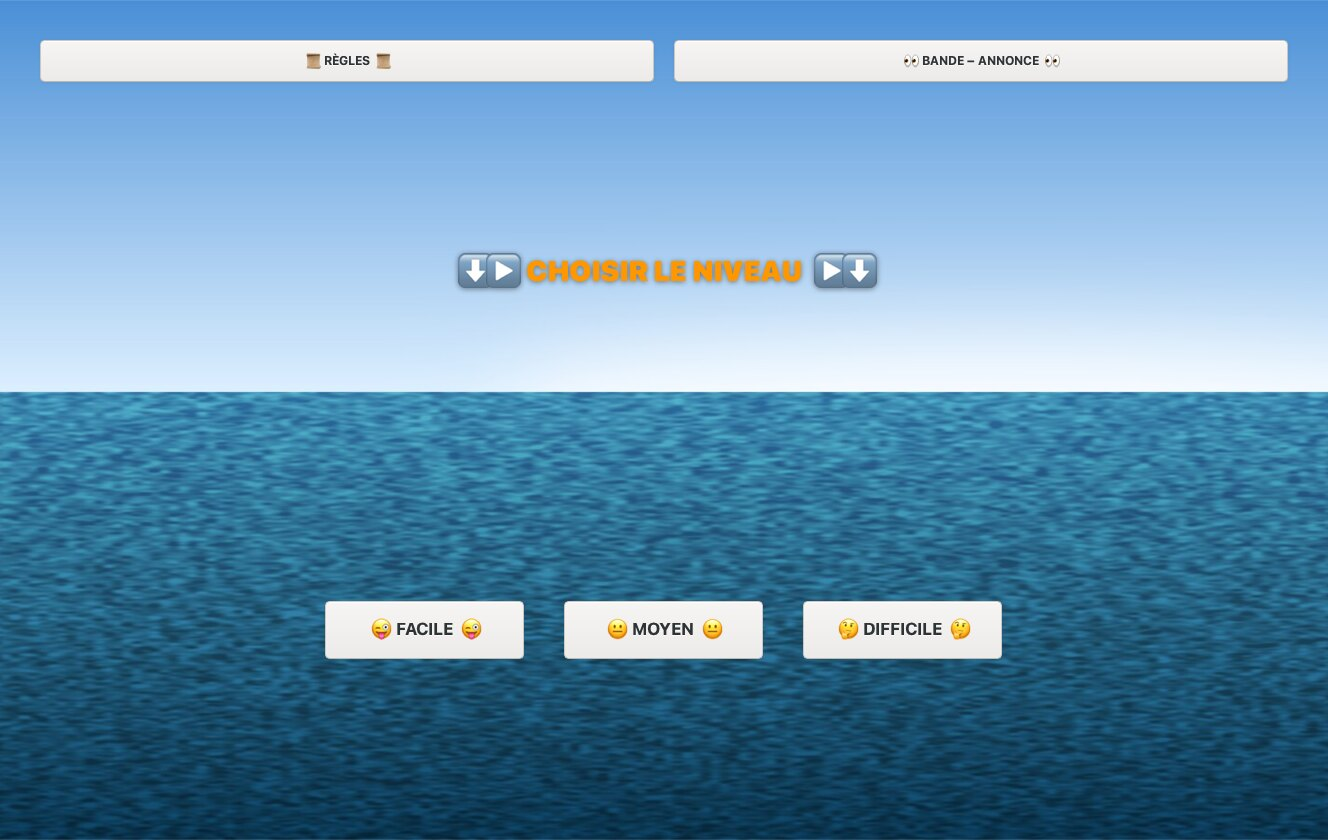
\includegraphics[width=0.78\textwidth]{../screenshots/menu.jpg}
    \caption{Version~2 --- choix du niveau.}
\end{figure}

\begin{figure}[H]
    \centering
    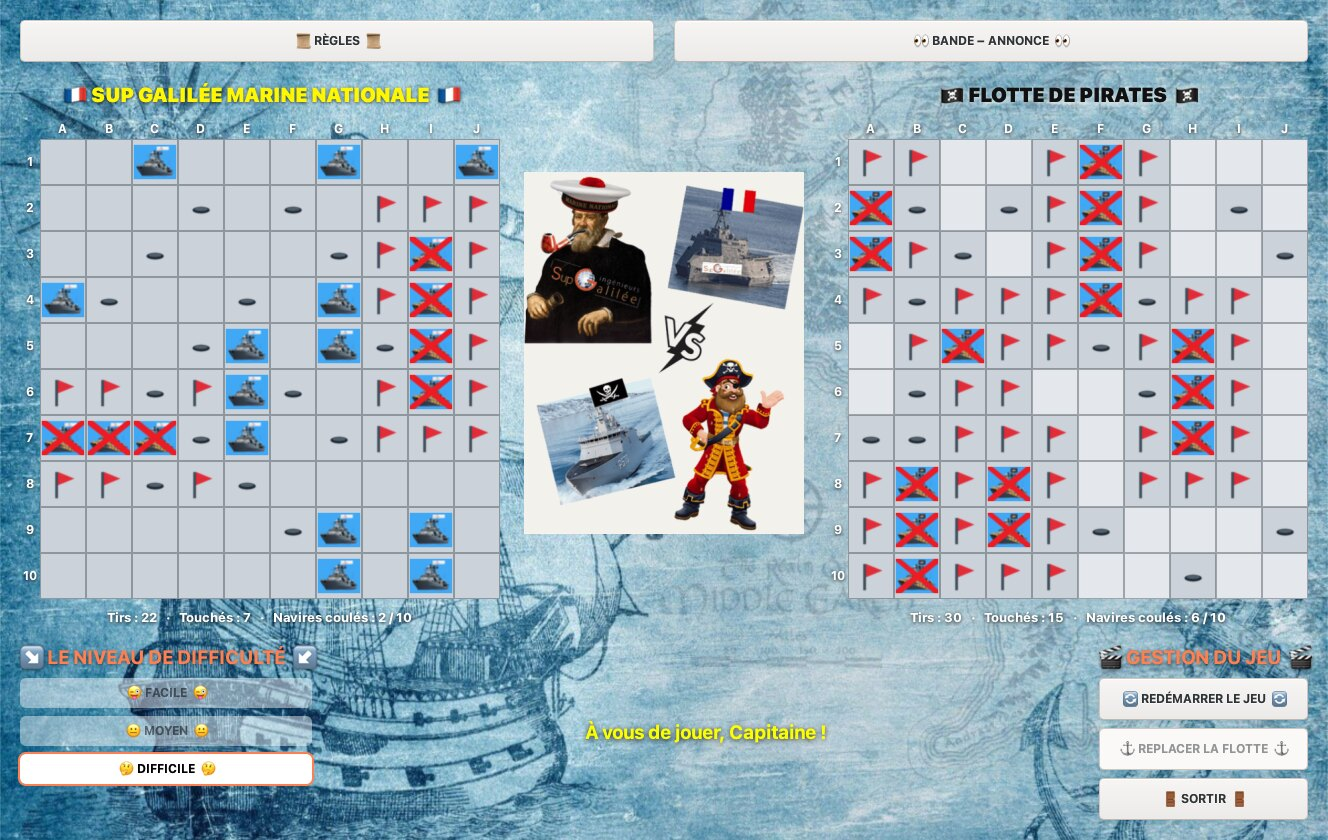
\includegraphics[width=\textwidth]{../screenshots/gameplay.jpg}
    \caption{Version~2 --- partie en cours au niveau difficile. À gauche, les drapeaux montrent
        ce que l'ordinateur a déduit ; à droite, ce que le joueur peut déduire.}
\end{figure}

\begin{figure}[H]
    \centering
    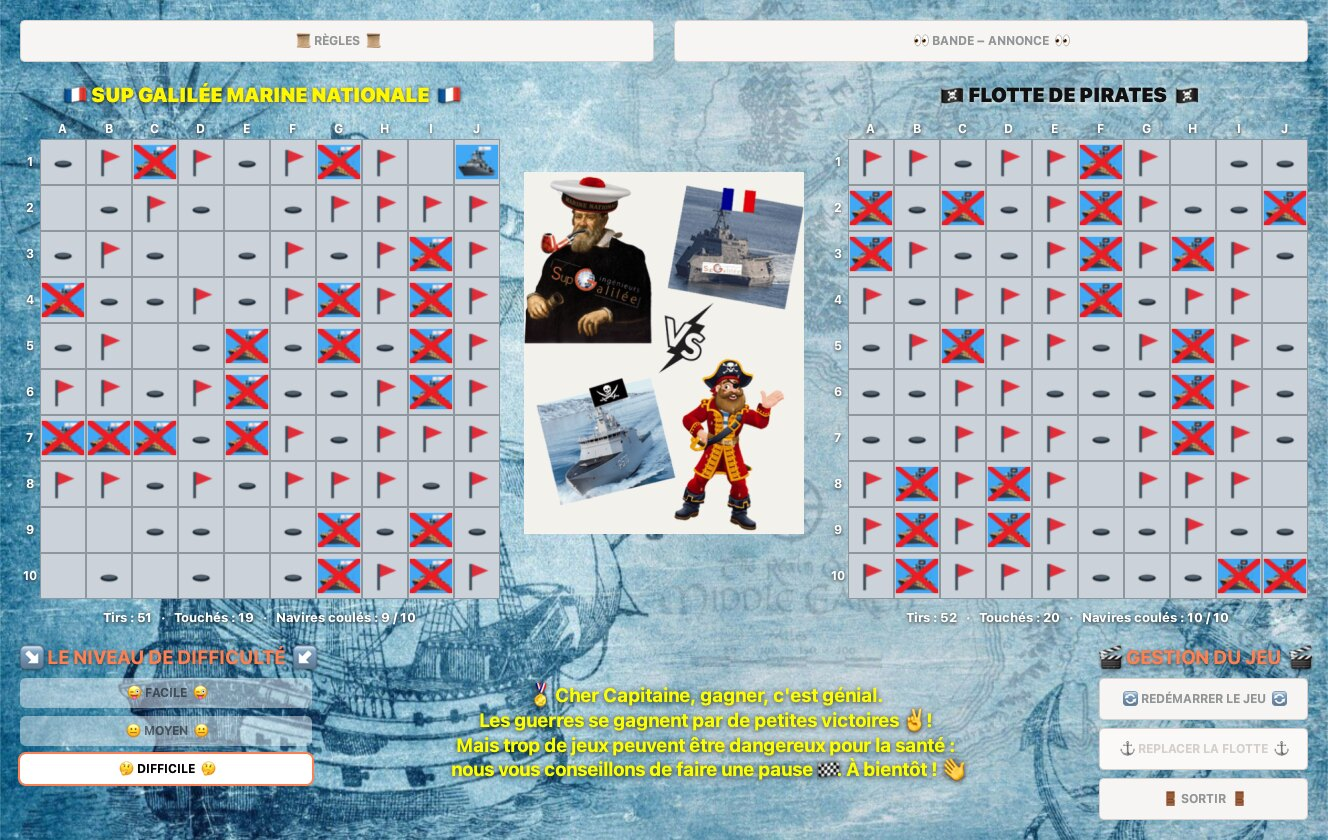
\includegraphics[width=\textwidth]{../screenshots/victory.jpg}
    \caption{Version~2 --- victoire.}
\end{figure}

\begin{figure}[H]
    \centering
    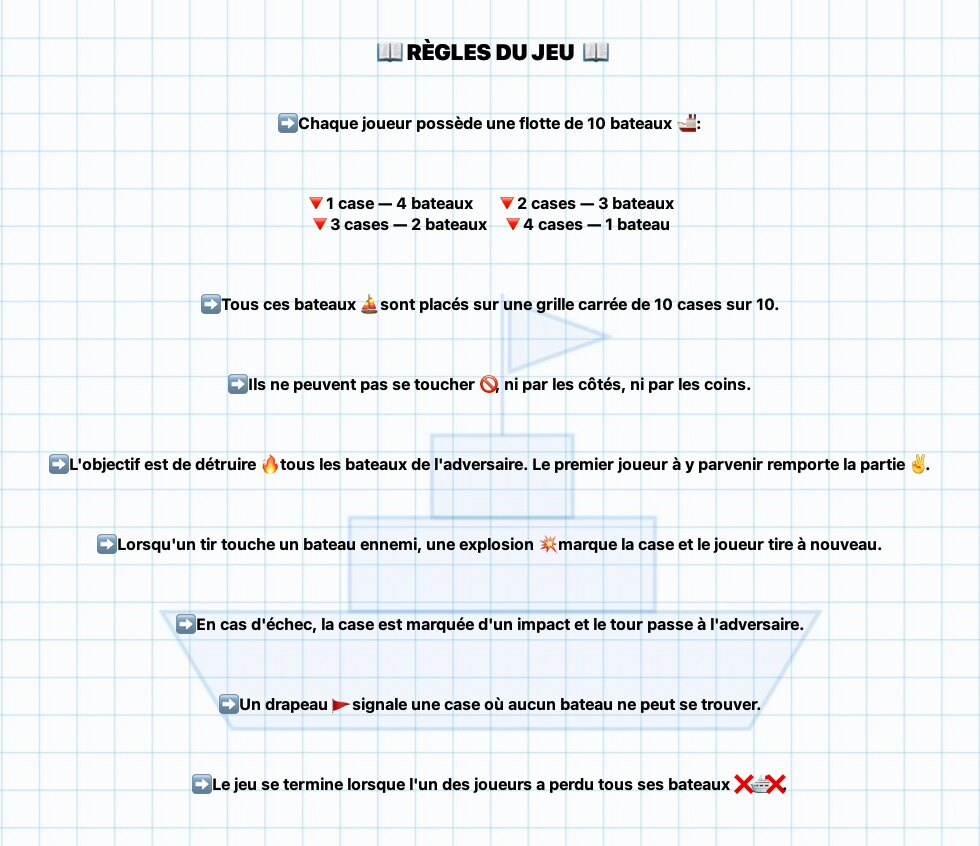
\includegraphics[width=0.8\textwidth]{../screenshots/rules.jpg}
    \caption{Version~2 --- fenêtre des règles.}
\end{figure}

\begin{figure}[H]
    \centering
    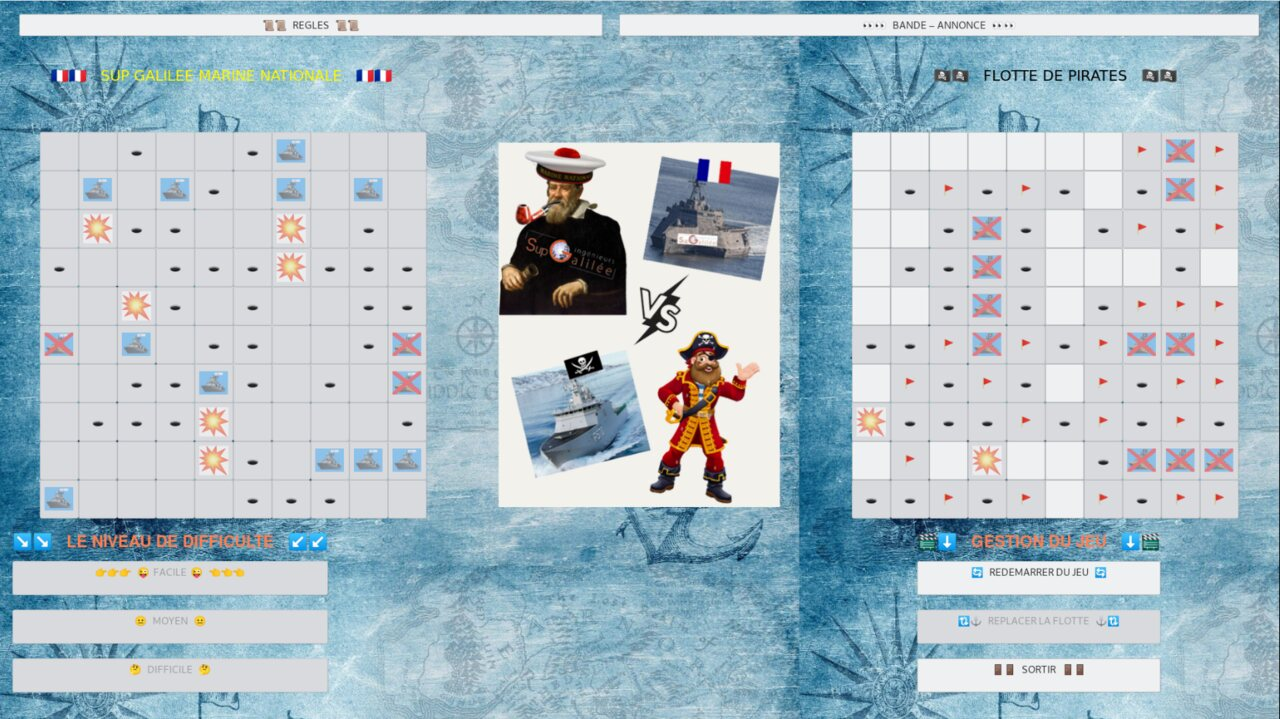
\includegraphics[width=\textwidth]{../screenshots/v1/gameplay.jpg}
    \caption{Version~1 (2023) --- partie en cours. L'identité visuelle a été conservée.}
\end{figure}
